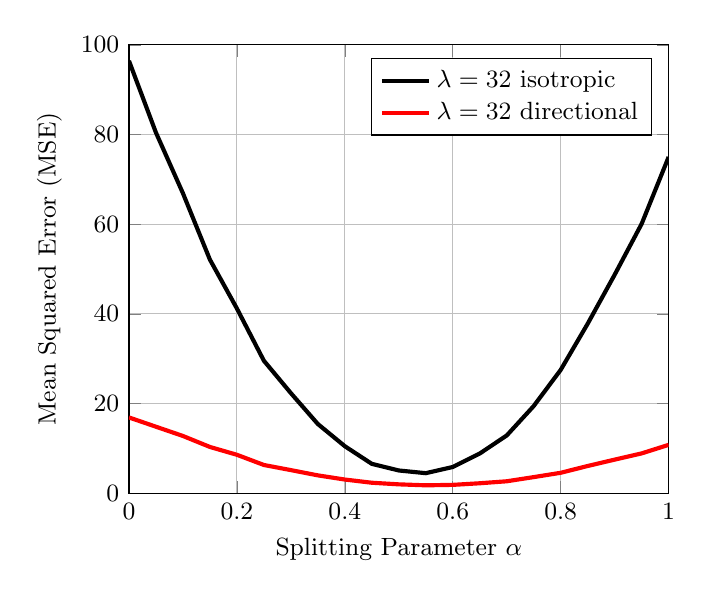
\begin{tikzpicture}
\begin{axis}[
font=\small,
xlabel= {Splitting Parameter $\alpha$},
ylabel= {Mean Squared Error (MSE)},
xmin = 0, xmax = 1,
ymin = 0, ymax = 100,
xmajorgrids,
ymajorgrids,
legend entries={$\lambda=32$ isotropic,$\lambda=32$ directional},
legend style={legend pos=north east,nodes=right}]

% Method: Bayes,
% Area Type = inscribed,
% Antenna Type = omnidirectional,
% Noise = 2,
% Trials = 50000,
% Total rate = 16,
% alpha_step =0.025,
% A_t =36.0,
% A_o =64.0,
% BMSE

\addplot [
color=black,
line width=1.5pt,
solid,
]
coordinates{
(0.0, 96.45209035)
(0.05, 80.42654262)
(0.1, 66.903744)
(0.15, 52.10264146)
(0.2, 41.20324598)
(0.25, 29.55163517)
(0.3, 22.33010006)
(0.35, 15.43733205)
(0.4, 10.49123755)
(0.45, 6.55550934)
(0.5, 5.07875978)
(0.55, 4.47613893)
(0.6, 5.85587843)
(0.65, 8.86221142)
(0.7, 12.88023637)
(0.75, 19.4563296)
(0.8, 27.5197941)
(0.85, 37.81174437)
(0.9, 48.74165857)
(0.95, 60.08816203)
(1.0, 74.99918686)
};

% Method: Bayes,
% Area Type = inscribed,
% Antenna Type = directional,
% Noise = 2,
% Trials = 50000,
% Total rate = 16,
% alpha_step =0.025,
% A_t =36.0,
% A_o =64.0,
% BMSE


\addplot [
color=red,
line width=1.5pt,
solid,
]
coordinates{
	(0.0, 16.90429818)
	(0.05, 14.83771601)
	(0.1, 12.77276452)
	(0.15, 10.3230366)
	(0.2, 8.5767891)
	(0.25, 6.30075548)
	(0.3, 5.15896029)
	(0.35, 3.98470553)
	(0.4, 3.05483395)
	(0.45, 2.34139352)
	(0.5, 1.98255413)
	(0.55, 1.76749939)
	(0.6, 1.86673371)
	(0.65, 2.22515382)
	(0.7, 2.66910387)
	(0.75, 3.59868373)
	(0.8, 4.56054986)
	(0.85, 6.07758196)
	(0.9, 7.49693503)
	(0.95, 8.88671712)
	(1.0, 10.7925513)
};

\end{axis}

\end{tikzpicture}

